\documentclass{article}

% using course specific template that adds section counting
\usepackage{../hw}

\renewcommand{\hmwkTitle}{Homework\ \#1}
\renewcommand{\hmwkDueDate}{January 23, 2020}
\newcommand{\prob}{\mathbb{P}}
\newcommand{\ind}{\mathbb{I}}

\begin{document}


\maketitle

\pagebreak

\setcounter{homeworkSectionCounter}{2}
\nobreak\extramarks{Problem \arabic{homeworkSectionCounter}.\arabic{homeworkProblemCounter}}{}\nobreak{}

\begin{homeworkProblem}[2][1]

Let $X, Y, Z$ be three disjoint subsets of random variables. We say $X$ and $Y$
are conditionally independent given $Z$ if and only if
$\mathbb{P}_{X, Y \mid Z}(x, y \mid z)
  = \mathbb{P}_{X \mid Z}(x \mid z) \mathbb{P}_{Y\mid Z}(y \mid z)$.
Show that $X$ and $Y$ are conditionally independent given $Z$ if and
only if the joint distribution for the three subsets of random variables factors
in the following form:
\[
  \mathbb{P}_{X, Y, Z}(x, y, z)=h(x, z) g(y, z)
\]

\solution

$(\Longrightarrow)$ If $ X \perp Y \mid Z$ then
\begin{align*}
  \mathbb{P}_{X,Y,Z} (x, y, z)
    &= \mathbb{P}_{X,Y\mid Z} (x,y \mid z) \mathbb{P}_Z(z) & \text{by Bayes Rule} \\
    &= \mathbb{P}_{X\mid Z}(x\mid z)\mathbb{P}_{Y\mid Z}(y\mid z)
  \mathbb{P}_Z(z) & \text{by conditional independence}\\
                  &= h(x,z) g(y,z)
\end{align*}
where $h(x,z) = \mathbb{P}_{X\mid Z}(x\mid z)$ and $g(y,z) = \mathbb{P}_{Y\mid
Z}(y\mid z) \mathbb{P}_Z(z)$.

$(\Longleftarrow)$ Conversely if there exist functions $h, g$ such that
$\mathbb{P}_{X,Y,Z} (x, y, z)= h(x,z) g(y,z)$, then
\begin{align*}
  \mathbb{P}_{X\mid Z}(x\mid z)
    &= \frac{ \mathbb{P}_{X,Z}(x,z) }{ \mathbb{P}_Z(z)}
    & \\
    &= \frac{ \sum_{y'}
    \mathbb{P}_{X,Y,Z}(x,y',z) }{ \sum_{x'} \sum_{y'} \mathbb{P}_{X,Y,Z}(x',y',z) }
      & \text{by law of total probability} \\
    &= \frac{ \sum^{}_{y'} h(x,z) g(y', z)}{ \sum^{}_{x'} \sum^{}_{y'} h(x',z)
      g(y',z)}
      & \\
    &= \frac{ h(x,z) \sum^{}_{y'} g(y', z)}{ \sum^{}_{x'} h(x',z)
      \sum^{}_{y'} g(y',z)}
      & \\
    &= \frac{ h(x,z)}{ \sum^{}_{x'} h(x',z)}
    & \numberthis \label{2-1-x-z}
\end{align*}
Of course an identical argument yields
\begin{align}
  \mathbb{P}_{Y\mid Z}(y\mid z)
    &= \frac{ g(y,z)}{ \sum^{}_{y'} g(y',z)}
    \numberthis \label{2-1-y-z}
\end{align}
Thus
\begin{align*}
\mathbb{P}_{X,Y \mid Z} (x,y \mid z)
  &= \frac{ \mathbb{P}_{X,Y,Z}(x,y,z)}{ \mathbb{P}_Z(z)} \\
  &= \frac{ \mathbb{P}_{X,Y,Z}(x,y,z)}{ \sum^{}_{x'} \sum^{}_{y'}
  \mathbb{P}_{X,Y,Z}(x',y',z)} \\
  &= \frac{ h(x,z) g(y,z) }{ \sum^{}_{x'} \sum^{}_{y'}
  h(x', z) g(y', z)} \\
  &= \frac{ h(x,z) g(y,z) }{ \sum^{}_{x'} h(x', z) \sum^{}_{y'}
  g(y', z)} \\
  &= \frac{ h(x,z) }{\sum^{}_{x'} h(x', z)}\frac{g(y,z) }{  \sum^{}_{y'}
  g(y', z)} \\
  &= \mathbb{P}_{X\mid Z}(x\mid z)\mathbb{P}_{Y\mid Z}(y\mid z)
\end{align*}
where the last equation follows from \eqref{2-1-x-z} and \eqref{2-1-y-z}. Of
course by definition this means $ X \perp Y \mid Z$. Notice that if these
random variables are continuous, replacing the summations with integrals will
also yield a valid argument.

\end{homeworkProblem}

\pagebreak

\begin{homeworkProblem}

In this problem, we will show by example that the distribution of a graphical
model need not have a factorization of the form in the Hammersley-Clifford Theorem if
the distribution is not strictly positive. In particular, we will consider a
distribution on the following simple 4-cycle where each node is a binary
\begin{center}
  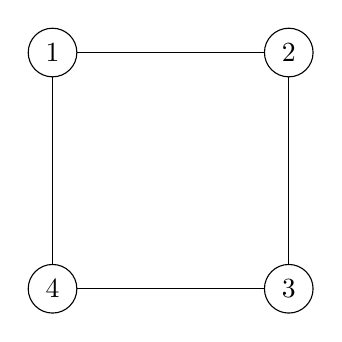
\begin{tikzpicture}[scale=3]
    \begin{scope}[every node/.style={circle,draw}]
      \node (4) at (0,0) {4};
      \node (3) at (1,0) {3};
      \node (1) at (0,1) {1};
      \node (2) at (1,1) {2};
    \end{scope}
    \draw (4) -- (3) -- (2) -- (1) -- (4);
  \end{tikzpicture}
\end{center}
random variable, $X_{i},$ for $i \in\{1,2,3,4\}$ Consider a probability
distribution that assigns a probability $1/8$ uniformly
to each of the following set of values $\left(X_{1}, X_{2},
X_{3}, X_{4}\right)$:
$$(0,0,0,0) \quad(1,0,0,0) \quad(1,1,0,0) \quad(1,1,1,0)$$
$$(0,0,0,1) \quad(0,0,1,1) \quad(0,1,1,1) \quad(1,1,1,1)$$
and assigns zero to all
other configurations of $\left(X_{1}, X_{2}, X_{3}, X_{4}\right)$.

\part

We first need to show that this distribution is Markov on our graph. To
do this, it should not be difficult to see that what we need to show are the following
conditions:
\begin{itemize}
  \item The pair of variables $X_{1}$ and $X_{3}$ are conditionally independent
    given $\left(X_{2}, X_{4}\right)$.
  \item The pair of variables $X_{2}$ and $X_{4}$ are conditionally independent
    given $\left(X_{1}, X_{3}\right)$.
\end{itemize}
First, show that if we interchange $X_{1}$ and $X_{4}$ and interchange $X_{2}$ and
$X_{3}$, we obtain the same distribution, i.e., $\mathbb{P}\left(x_{1}, x_{2},
x_{3}, x_{4}\right)=\mathbb{P}\left(x_{4}, x_{3}, x_{2}, x_{1}\right)$. This
implies that if we can show the first condition, then the other is also true.

\solution

Let $Y$ denote the set of values above, such that $ \mathbb{P}(Y) = \qty{
\frac{1}{8} } $ and $ \mathbb{P}(\mathcal{X}^4 \setminus Y) = \qty{ 0 }. $
Let $\pi$ denote the reversal operation
\[\pi(x_1,x_2,x_3,x_4) = (x_4, x_3, x_2, x_1)\]
which is a bijection on $\mathcal{X} ^ 4$. Notice that $\pi$ is closed on $Y$ and on
$\mathcal{X}^4 \setminus Y$. Then it becomes immediately clear that
\begin{align*}
  \mathbb{P}(\pi(x)) &= \frac{1}{8} = \mathbb{P}(x) \quad\text{ for all } x \in Y \\
  \mathbb{P}(\pi(x)) &= 0 = \mathbb{P}(x) \quad \text{ for all } x \notin Y
\end{align*}
and we conclude $ \mathbb{P}(\pi(x)) = \mathbb{P}(x) $ for all $x \in \mathcal{X}^4$.

\pagebreak

\part

Show that whatever pair of values you choose for $\left(X_{2},
X_{4}\right)$, we then know either $X_{1}$ or $X_{3}$ with certainty. For
example, $\left(X_{2}=0, X_{4}=0\right)$ implies that $X_{3}=0 .$ Since we know
either $X_{1}$ or $X_{3}$ with certainty, then conditioning on the other one of
these obviously provides no additional information, trivially proving
conditional independence.

\solution

There are only four cases so we'll enumerate them:
\begin{align*}
  ( X_2, X_4) = (0, 0) \implies X_3 = 0 \\
  ( X_2, X_4) = (1, 1) \implies X_3 = 1 \\
  ( X_2, X_4) = (1, 0) \implies X_1 = 1 \\
  ( X_2, X_4) = (0, 1) \implies X_1 = 0
\end{align*}
Each of these implications follows from the distribution, eliminating the
values not in $Y$ which have probablity zero. Notice in the first two cases, we
know $X_3$ completely, and so trivially $X_1$ is independent of $X_3$ given
these values of $(X_2,X_4)$. Similarly in the last two cases, we know $X_1$
completely, so trivially $X_3$ is independent of $X_1$ given these values of
$(X_2, X_4)$. Thus, in any case,
\[X_1 \perp X_3 \mid (X_2, X_4)\]
and by the symmetry in part (a) we can also conclude
\[X_2 \perp X_4 \mid (X_1, X_3).\]

\part

What we now need to show is that the distribution cannot be factorized in the
way stated in the Hammersley-Clifford Theorem. We will do this by contradiction.
Noting that the maximal cliques in our graph are just the edges and absorbing
the normalization constant $ \frac{1}{Z} $ into any of the pairwise
compatibility functions, we know that if our distribution has the factorization
implied by the Hammersley-Clifford Theorem, we can write it in the following
form:
\[
  \mathbb{P}(x_1,x_2,x_3,x_4) = \psi_{12}(x_1,x_2)\psi_{23}(x_2,x_3)\psi_{34}(x_3,x_4)\psi_{41}(x_4,x_1)
\]
Show that assuming that our distribution has such a factorization leads to a
contradiction by examining the values of $ \mathbb{P}(0,0,0,0)$,
 $\mathbb{P}(0,0,1,0)$, $\mathbb{P}(0,0,1,1)$, and $\mathbb{P}(1,1,1,0)$.

\solution

As noted above, we observe that the cliques in this graph are precisely the
edges
\[\{1,2\}, \{2,3\}, \{3,4\}, \{4,1\}\]
and, assuming the Hammersley-Clifford Theorem factorization holds, we can write
\[ \mathbb{P}(x_1, x_2, x_3, x_4)
= \frac{1}{Z}
\widetilde{\psi}_{12}(x_1,x_2)\psi_{23}(x_2,x_3)\psi_{34}(x_3,x_4)\psi_{41}(x_4,x_1).\]
Define $\psi_{12}(x_1,x_2) = \frac{1}{Z}\widetilde{\psi}_{12}(x_1,x_2)$
so that we have
\[ \mathbb{P}(x_1, x_2, x_3, x_4)
= \psi_{12}(x_1,x_2)\psi_{23}(x_2,x_3)\psi_{34}(x_3,x_4)\psi_{41}(x_4,x_1).\]

Next, notice that because
\[0 = \mathbb{P}(0,0,1,0) =
  \psi_{12}(0,0)\psi_{23}(0,1)\psi_{34}(1,0)\psi_{41}(0,0)
\]
it must be the case that one of the factors
$\psi_{12}(0,0)$, $\psi_{23}(0,1)$, $\psi_{34}(1,0)$, $\psi_{41}(0,0)$ is
equal to zero. However,
\[ \frac{1}{8} = \mathbb{P}(0,0,0,0) =
  \psi_{12}(0,0)\psi_{23}(0,0)\psi_{34}(0,0)\psi_{41}(0,0)
\]
implies that neither $\psi_{12}(0,0)$ nor $\psi_{41}(0,0)$ is zero. Similarly
\[ \frac{1}{8} = \mathbb{P}(0,0,1,1) =
  \psi_{12}(0,0)\psi_{23}(0,1)\psi_{34}(1,1)\psi_{41}(1,0)
\]
and
\[ \frac{1}{8} = \mathbb{P}(1,1,1,0) =
  \psi_{12}(1,1)\psi_{23}(1,1)\psi_{34}(1,0)\psi_{41}(0,1)
\]
imply that $\psi_{23}(0,1)$ and $\psi_{34}(1,0)$ are nonzero, respectively. Thus
we have reached a contradiction, and conclude that the Hammersley-Clifford
Theorem factorization does not hold for this distribution.

\end{homeworkProblem}

\begin{homeworkProblem}
Given a graph $G=(V,E)$, an {\em independent set} of $G$ is a subset $S\subseteq V$
of the vertices, such that no two vertices in $S$ is connected by an edge in $E$.
Precisely, if $i,j\in S$ then $(i,j)\notin E$.
We let $\mathrm{IS}(G)$ denote the set of all independent sets of $G$,
and let $Z(G)=|\mathrm{IS}(G)|$ denote its size, i.e. the total number of independent sets in $G$.
The number of independent sets $Z(G)$ is at least $1+|V|$,
since the empty set and all subsets with single vertex are always independent sets.
We are interested in the uniform probability measure over $S$:
\begin{eqnarray*}
	\prob_{\mathrm{IS}(G)}(S) = \frac{1}{Z(G)}\ind(S\in\mathrm{IS}(G))\;,
\end{eqnarray*}
where $\ind(A)$ is an indicator function which is one if event $A$ is true and zero if false.

\part

The set $S$ can be naturally encoded by a binary vector $x\in\{0,1\}^{|V|}$ by letting $x_i=1$ if and only if $i\in S$.
Denote by $\prob_G(x)$ the probability distribution induced on this vector $x$
according to $\prob_{\mathrm{IS}(G)}(S)$. Show that $\prob_G(x)$ is a pairwise graphical model on $G$.

\solution

Immediately from the definition of an independent set, we have $S
\subseteq V $ is independent if and only if $x_i = x_j = 1$ implies $(i,j)
\notin E$. Notice we can define factors by using the contrapositive of this
statement: $S$ is independent iff $(i,j) \in E$ implies at least one of
$x_i$, $x_j$ is not 1. Thus, for every $(i,j) \in E$, define
\[
  \psi_{i,j}(x_i,x_j) =
    \begin{cases}
      0 &\text{ if }x_i = x_j = 1 \\
      1 &\text{ otherwise }
    \end{cases}
\]
Now it is evident that $\ind(S) = \prod_{(i,j)\in E}\psi_{i,j}(x_i,x_j)$.
Letting $Z = Z(G)$ we have
\[
  \prob_G(x)=(1/Z)\prod_{(i,j)\in E}\psi_{i,j}(x_i,x_j)
\]
and therefore $\prob_G(x)$ is a pairwise graphical model on $G$.

\pagebreak

\part

Let $L_n$ be the line graph with $n$ vertices, i.e. the graph with vertex set
$V(L_n)=\{1,2,3,\ldots,n\}$ and edge set $E(L_n)=\{(1,2),(2,3),\ldots,(n-1,n)\}$.
Derive a formula for $Z(L_n)$.

\solution

In the first two cases $n = 0,1$, there are
no edges and it is easy to see each subset is independent, i.e. $L_0 = 1$ and
$L_1 = 2$. For $n > 1$ consider partitioning the independent sets
$\mathrm{IS}(L_n)$ by the inclusion or exclusion of the last vertex $n$.
Geometrically it is clear that $S \subseteq V$ is independent iff there are no consecutive vertices $k, k+1 \in S$.
So if $S$ is independent and $n \in S$, this necessitates $n-1 \notin S$, while
the other vertices $\qty{1,\ldots, n-2}$ can vary subject to independence in
$L_{n-2}$. Similarly if $S$ is independent and $n \notin S$, then the other
vertices $\qty{1,\ldots, n-1}$ can vary subject to independence in $L_{n-1}$.
Therefore
\begin{align*}
  Z(L_n)
     = \abs{\mathrm{IS}(L_n)}
    &= \abs{
             \qty{S \in \mathrm{IS}(L_n): n \in S}
        \cup \qty{S \in \mathrm{IS}(L_n): n \notin S}
          } \\
    &= \abs{\qty{S \in \mathrm{IS}(L_n): n \in S}}
     + \abs{\qty{S \in \mathrm{IS}(L_n): n \notin S}} \\
    &= Z(L_{n-2}) + Z(L_{n-1})
\end{align*}
from which it is clear that $Z(L_n)$ is simply an offset of the Fibonacci
sequence $0,1,1,2,3,5\ldots$, namely $Z(L_n) = F_{n+2}$. Of course we can use
the commonly known matrix exponentiation formula
\[
  \mqty(1 & 1 \\ 1 & 0)^n = \mqty(F_{n+1} & F_n \\ F_n & F_{n-1})
\]
to derive
\[
  Z(L_n) = \qty(\mqty(1 & 1 \\ 1 & 0)^{n+1})_{1,1}
\]

\part

With the above definitions, derive a formula for $\prob_{L_n}(x_i=1)$, for each $i\in\{1,\ldots,n\}$.
Plot $\prob_{L_n}(x_i)$ versus $i$ for $n=11$. Describe the main features of this plot.
Can you give an intuitive explanation?

\solution

For any $i \in \qty{1,\ldots n}$ clearly the uniform distribution implies
\[
  \prob_{L_n}(x_i = 1) = \frac{\abs{\qty{S \in \mathrm{IS}(L_n): i \in S}}}{Z(L_n)},
\]
that is, $\prob_{L_n}(x_i = 1)$ is simply the proportion of independent sets
containing the vertex $i$. To derive a formula, it is easiest to first consider
the endpoints, so consider when $i=n$. Recall above when we expressed the
number of independent sets
$Z(L_n)$ by the sum of the number of independent sets including and
excluding vertex $n$, of which there are $Z(L_{n-2})$ and $Z(L_{n-1})$
respectively. A symmetric argument applies to the vertex $1$, such that
\[
  \prob(x_1 = 1) = \prob(x_n = 1) = \frac{Z(L_{n-2})}{Z(L_n)}.
\]
For $n>2$ and $1 < k < n$ we can apply similar reasoning: the presence of node
$k$ implies the exclusion of nodes $k-1, k+1$, while the vertices
$\qty{1,\ldots,k-2}$ and $\qty{k+2,\ldots,n}$ can vary subject to independence
in $L_{k-2}$ and $L_{n-(k+1)}$ respectively. Therefore
\[
  \prob(x_k = 1) =
  \frac{
    Z(L_{k-2}) Z(L_{n-k-2})
  }{
    Z(L_n)
  }
  \numberthis \label{2-3}
\]
and notice if we define $Z(L_{-2}) \triangleq 1$ and $Z(L_{-1}) \triangleq 1$ we
can use \eqref{2-3} as a general formula for $k=1,\ldots,n$ and $n>0$.

\pagebreak

The plot is shown below.

\begin{figure}[h!]
\begin{center}
  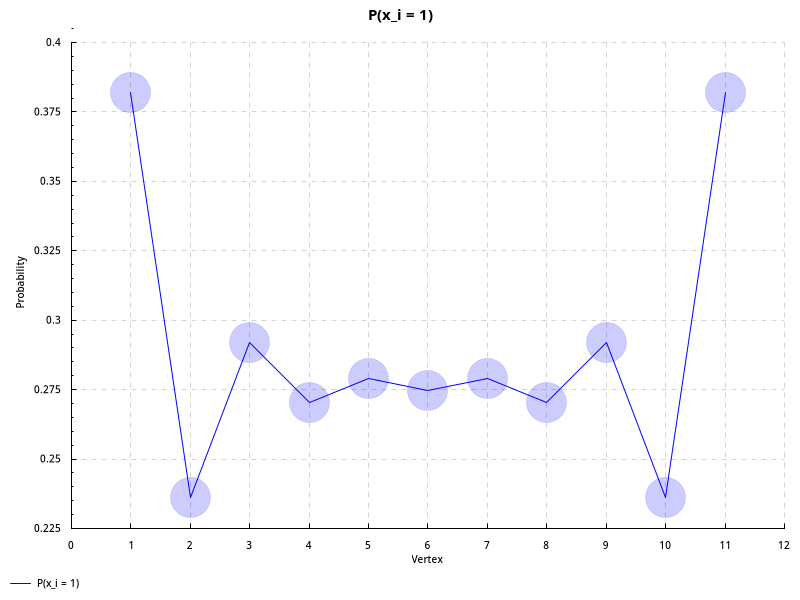
\includegraphics[width=\linewidth]{problem_2-3-c.png}
\end{center}
\caption{$\prob_{L_n}(x_i)$ versus $i$ for $n=11$}
\label{fig:2-3-c}
\end{figure}

Because of the rate at which the Fibonacci sequence increases, it makes sense
that $Z(L_{n-2})$ is larger than the product of the smaller numbers $Z(L_{k-2})
Z(L_{n-k-2})$, hence the peaks at the endpoints of the graph.

\pagebreak

\part

The same probability distribution $\prob_{L_n}(x)$ can be also represented with a Bayesian network.
For example, $\prob_G(x)=\prob_{X_1}(x_1)\prob_{X_2|X_1}(x_2|x_1)\prob_{X_3|X_1,X_2}(x_3|x_1,x_2)\cdots\prob_{X_{11}|X_1\cdots X_{10}}(x_{11}|x_1\cdots x_{10})$.
Using the recursions used in $(b)$ and $(c)$, write the conditional probability distributions for this Bayesian network.

\solution

Since each node only depends on its immediate parent, we have

\begin{align*}
  \prob_{L_n}(x)
    &= \prob_{X_1}(x_1)\prod_{k=2}^n \prob_{X_k \mid X_1,\ldots X_{k-1}}(x_k \mid
        x_1,\ldots,x_{k-1}) \\
    &= \prob_{X_1}(x_1)\prod_{k=2}^n \prob_{X_k \mid X_{k-1}}(x_k \mid x_{k-1}).
\end{align*}

To calculate $\prob_{X_k \mid X_{k-1}}(x_k \mid x_{k-1})$ we apply the same
reasoning as above. When $k-1 \in S$ we immediately know $k \notin S$. On the
other hand supposing that node $k-1 \notin S$, the probability that $k
\in S$ is the same as the probability that the first vertex $k$ is in an independent
set in the subgraph of nodes $\qty{k, \ldots, n}$ of size $n-k+1$. That is,
\[ \prob_{X_k \mid X_{k-1}} (x_k = 1 | x_{k-1} = 0) = \prob_{L_{n-k+1}}(x_1 = 1)
= \frac{Z(L_{n-k-1})}{Z(L_{n-k+1})} \]
which follows from our general formula for $\prob_{L_n}(x_1 = 1)$ in part (c).
Putting it all together we have derived
\[ \prob_{X_k \mid X_{k-1}} (x_k = 1 | x_{k-1})
  = \begin{cases}{}
    0 &\text{ if } x_{k-1} = 1 \\
    \frac{Z(L_{n-k-1})}{Z(L_{n-k+1})} &\text{ otherwise }
  \end{cases}
\]
for $k = 2,\ldots, n$.

\end{homeworkProblem}
\pagebreak
\begin{homeworkProblem}

We again consider the independent set explained in the previous problem.
Now let $G=T_{k,\ell}$ denote the rooted tree with branching factor $k$ and $\ell$ generations,
that is the root has $k$ descendants and each other node has one ancestor and $k$ descendants except for the leaves.
The total number of vertices is $(k^{\ell+1}-1)/(k-1)$, and $T_{k,\ell=0}$ is the graph consisting only of the root.
We let $\phi$ denote the root of $T_{k,\ell}$.

\part

Let $Z_\ell=Z(T_{k,\ell})$ denote the total number of independent sets of $G=T_{k,\ell}$.
Let $Z_{\ell}(0)$ be the number of independent sets in $T_{k,\ell}$ such that the root is $x_\phi=0$,
and $Z_{\ell}(1)$ be the number of independent sets such that $x_\phi=1$. It is immediate that
$Z_0(0)=Z_0(1)=1$. Derive a recursion expressing $(Z_{\ell+1}(0),Z_{\ell+1}(1))$
as a function of $(Z_\ell(0),Z_\ell(1))$.

\solution

If $x_\phi = 0$, this imposes no restrictions on its $k$ descendant subgraphs,
each of which is isomorphic to
$T_{k, \ell-1}$. Since these subgraphs are not connected, the total number of
independent sets $Z_\ell(0)$ is the same as the $k$-product of the number of independent
sets in each $T_{k, \ell-1}$ subgraph. Therefore
\[ Z_\ell(0) = \qty(Z_{\ell-1}(0) + Z_{\ell-1}(1))^k. \]
If $x_\phi = 1$, this imposes the restriction that each of its immediate
children is zero. Again since these $k$ immediate children are themselves roots
of $T_{k, \ell-1}$ subgraphs and these subgraphs are not connected to one
another, we have
\[ Z_\ell(1) = \qty(Z_{\ell-1}(0))^k. \]
Formally we have
\begin{align*}
                \qty( Z_0(0), Z_0(1) ) &= \qty( 1, 1 ) \\
  \qty( Z_{\ell+1}(0), Z_{\ell+1}(1) ) &= \qty( \qty(Z_{\ell}(0) +
  Z_{\ell}(1))^k, \qty(Z_{\ell}(0))^k ).
\end{align*}

\part

Using the above recursion, derive a recursion for the probability that the root
belongs to a uniformly random independent set. Explicitly, derive a recursion for
\begin{eqnarray*}
p_\ell &=& \prob_{T_{k,\ell}}(\{x_\phi=1\})\;.
\end{eqnarray*}

\solution

Given that the distribution is uniform we simply need the proportion of
independent sets with $x_\phi = 1$. Therefore $p_0 = \frac{1}{2}$ and for $\ell
\geq 0$
\begin{align*}
  p_\ell &= \frac{Z_\ell(1)}{Z_\ell(0)+Z_\ell(1)}
          = 1 - \frac{Z_\ell(0)}{Z_\ell(0)+Z_\ell(1)} \\
  p_{\ell+1} &= \frac{Z_{\ell+1}(1)}{Z_{\ell+1}(0)+Z_{\ell+1}(1)} \\
             &= \frac{Z_\ell(0)^k}{\qty(Z_\ell(0)+Z_\ell(1))^k + Z_\ell(0)^k} \\
             &= \frac{1}{\qty( \frac{Z_\ell(0)+Z_\ell(1)}{Z_\ell(0)})^k + 1} \\
             &= \frac{1}{\qty( \frac{1}{1-p_\ell})^k + 1}.
\end{align*}

\part

Program this recursion and plot $p_\ell$ as a function of $\ell\in\{0,1,\ldots,50\}$
for four values of $k$, e.g. $k\in\{1,2,3,10\}$.
Comment on the qualitative behavior of these plots.

\part

Prove that, for $k\leq 3$, the recursion converges to a unique value using Banach's fixed point theorem.

\end{homeworkProblem}

\end{document}
